Several test facilities at the Max-Planck-Institut f\"ur Physik, Munich, were founded for the research and development of segmented $n$-type germanium detectors for the Phase~II of the GERDA experiment. Based on them the operation and performance of several segmented detectors in vacuum as well as in cryogenic liquid have been systematically examined; various data samples have been taken to investigate the event discrimination power of segmented germanium detectors. A brief introduction of these test facilities is given in this chapter. The studies and analysis based on them are described in the following chapters.

\section{Phase~II prototype detectors} 
\label{sec:tt:dets} 
The first two prototype detectors for GERDA Phase~II have been developed and produced in close collaboration with the manufacturer Canberra-France, and called \emph{Siegfried} I and \emph{Siegfried} II. The \emph{Siegfried} series are $n$-type true coaxial cylindrical crystals made of natural germanium with a height of 70~mm and a diameter of 75~mm with a 10~mm hole in the center. The active volume is 302~cm$^{3}$, the total mass is 1.6~kg. They are 18-fold segmented with a 6-fold segmentation in the azimuthal angle $\phi$ and a 3-fold segmentation in the height $z$.  The segmentation scheme and the detector coordinate system are displayed in Fig.~\ref{fig:tt:segm} where a scheme of the cabling (left) and the segment numbering (right) are shown. The segments are read out using a Kapton flexible printed-circuit-board (FPCB) with snap-contacts~\cite{Sie07}. Pictures of the two detectors together with the contact cables are shown in Fig.~\ref{fig:tt:sies}. The detector specifications as provided by the
\mbox{manufacturer} are summarized in
Table~\ref{tab:tt:detpar}. 
\begin{figure}[tbhp]
  \centering
  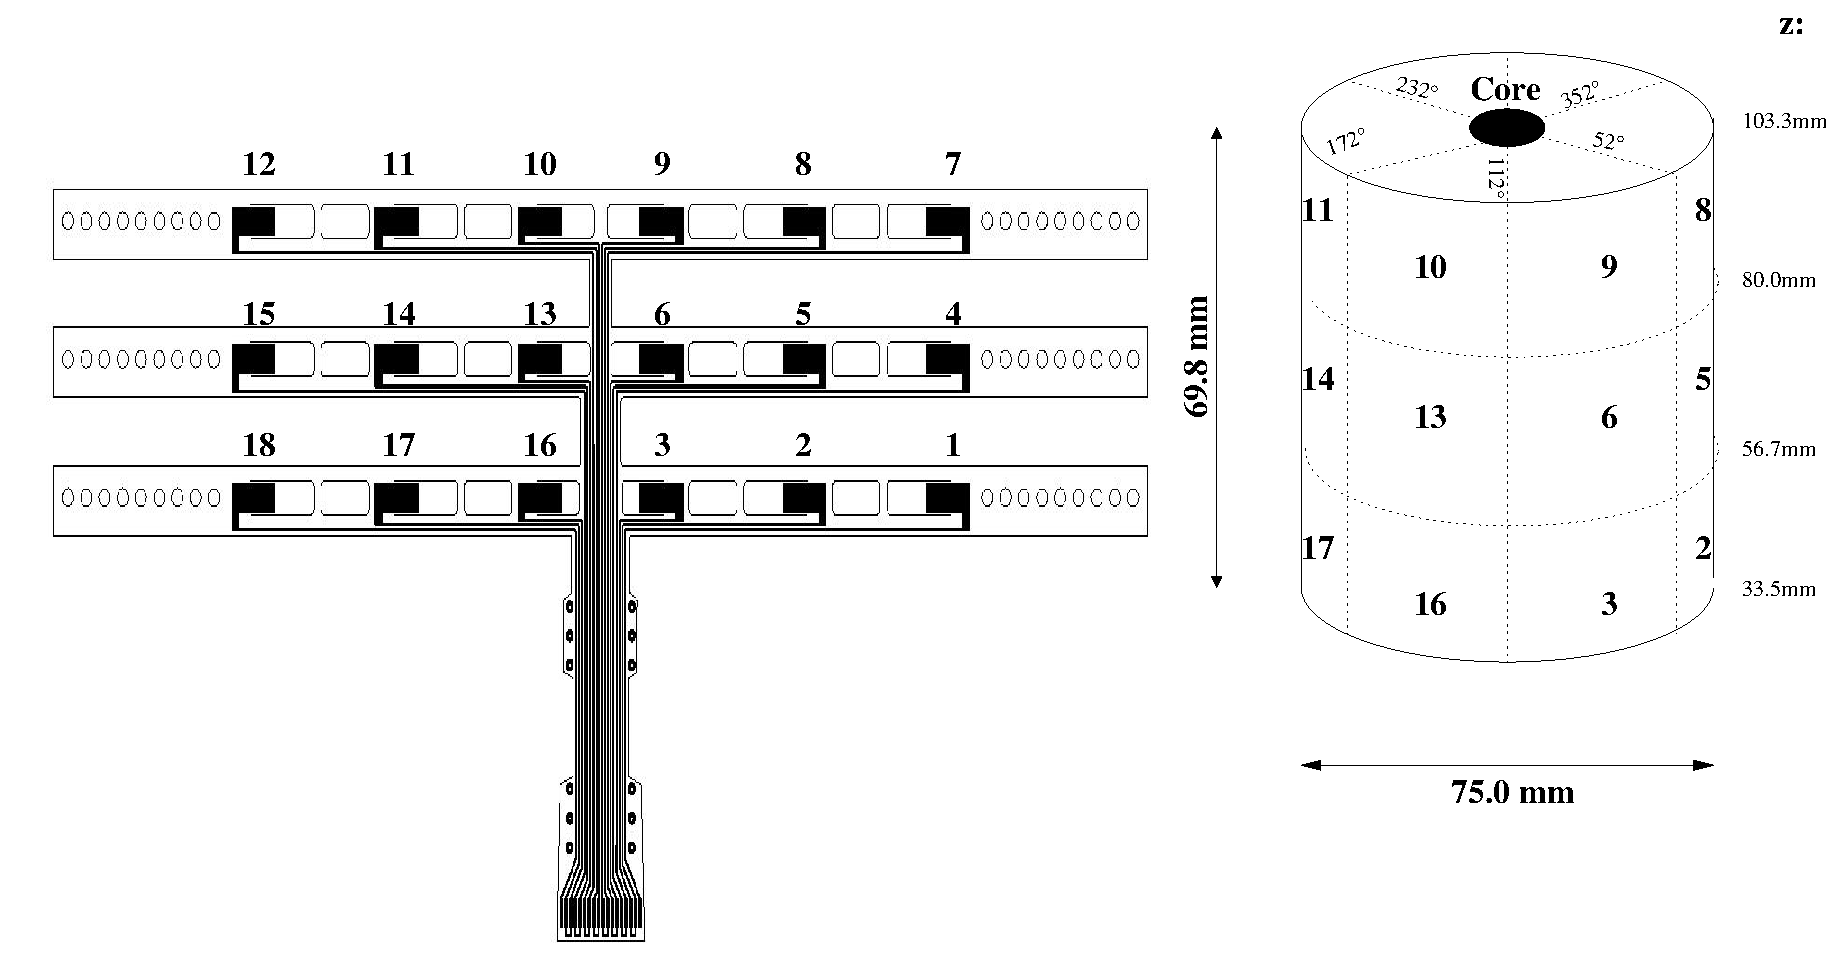
\includegraphics[width=0.95\textwidth]{segmentation_scheme}  
  \caption{Cabling scheme (left) and segment numbering (right) of the     prototype detector.}
  \label{fig:tt:segm}
\end{figure}

\begin{figure}[tbhp]
  \centering
  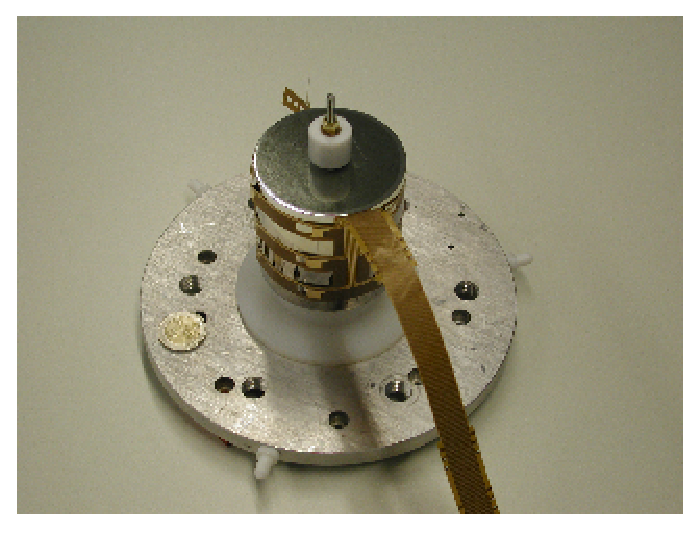
\includegraphics[height=0.25\textheight]{SiegfriedI}\hfil
  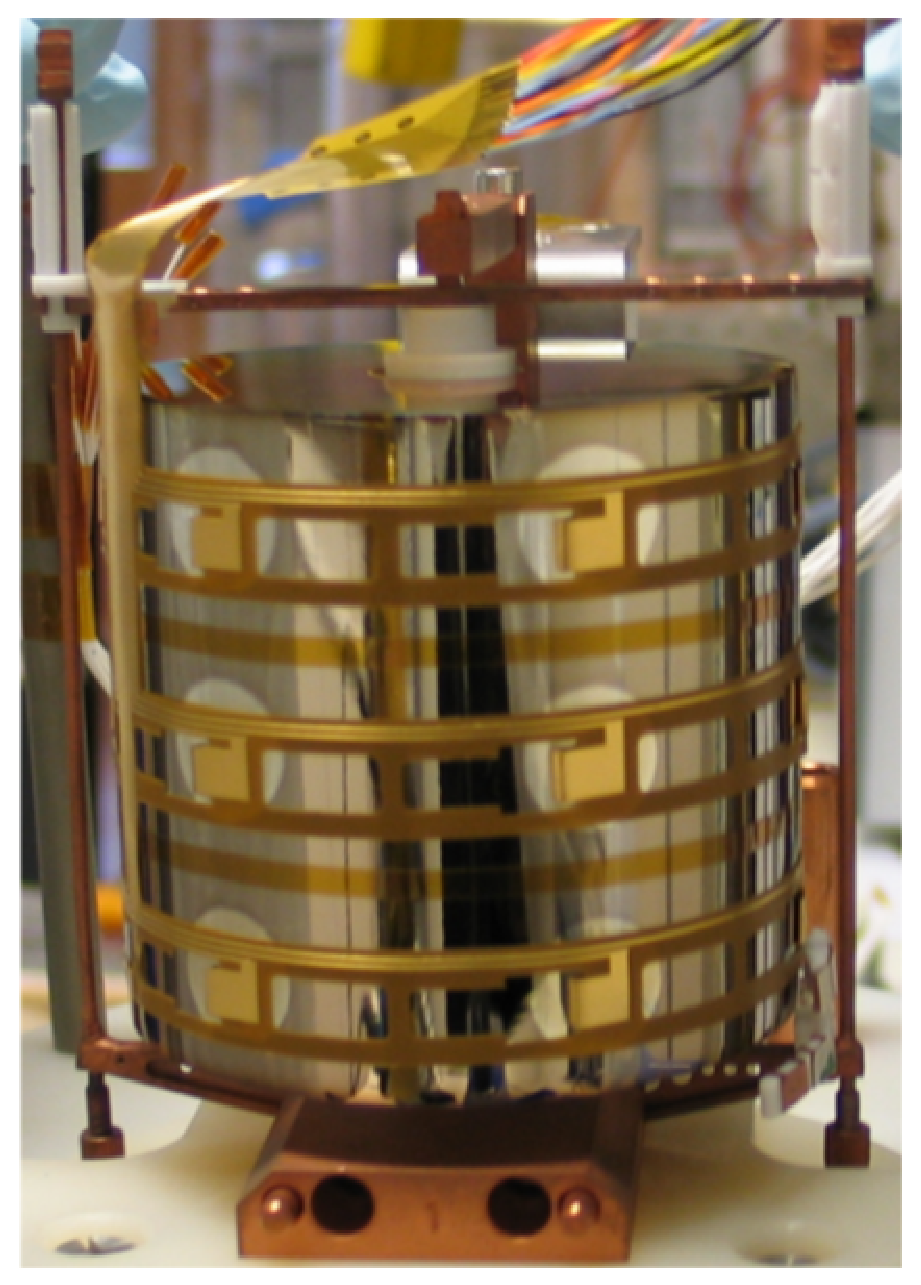
\includegraphics[height=0.25\textheight]{SiegfriedII}
\caption{Siegfried I mockup (left) and Siegfried II (right) with Kapton FPCB contact cables around.}
\label{fig:tt:sies}
\end{figure}

\begin{table}[tbhp]
\centering
\caption{Detector specifications as provided by the manufacturer.}
\label{tab:tt:detpar}
\begin{tabular}{lll}\\\hline
Parameter & \emph{Siegfried} I  & \emph{Siegfried} II \\\hline
Outer diameter (mm)   & 75.0 & 75.2\\ 
Inner diameter (mm)   & 10 & 10 \\ 
Height (mm)           & 69.8 & 70.2 \\\hline 
Operating voltage (V) & +3000 & +2000 \\ 
FWHM at 122~keV (keV)  & 0.99 & 0.96 \\ 
FWHM at 1333~keV (keV) & 1.99 & 2.11 \\ \hline 
\end{tabular}
\end{table}


\section{Cryostats}
\label{sec:tt:cryo}

\subsection{Commercial cryostat}
\label{sec:tt:comc}
\emph{Siegfried} I was delivered with a commercial cryostat as shown in the left picture of Fig.~\ref{fig:tt:comcryo}. It was placed inside a two-walled aluminum vacuum can with a combined thickness of 6~mm. The detector center is at $z=66$~mm and $r=0$~mm, the vacuum can extends up to $z=116$~mm and $r=75$~mm. A copper cooling finger was used as thermal link between the detector and a 60~l dewar below the detector filled will liquid nitrogen. A temperature monitor was used to measure the temperatures at several locations in the detector cryostat using Pt100 resistors. Liquid nitrogen was refilled daily resulting in a temperature stability of about $\pm3$~K. A comparison of spectra taken at different temperatures within this range showed neither significant differences in the general shape of the spectra nor in the energy resolution.

The core and each segment of \emph{Siegfried} I were read out through two massive copper tubes on both sides of the vacuum can housing front-end electronics as shown in the right picture of Fig.~\ref{fig:tt:comcryo}. The left side provided the feed-throughs for the high voltage and the signal lines for segments~10--18, the right side serviced the signal lines for segments~1-7 and housed a multi-purpose connector for the signal lines for segments~8--9 and a test-input for the core pre-amplifier.

\begin{figure}[tbhp]
  \centering
  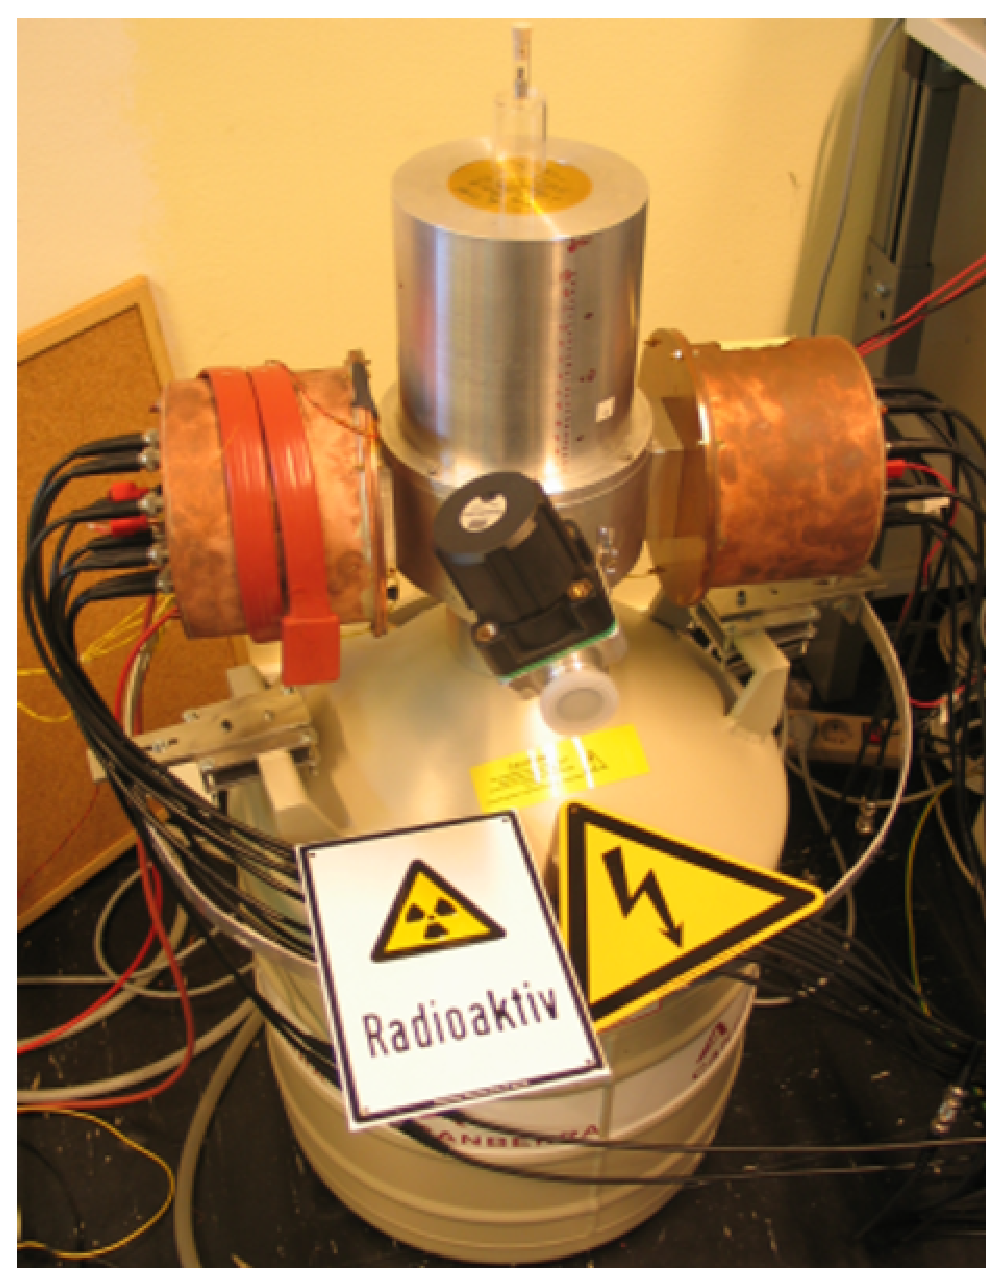
\includegraphics[height=0.25\textheight]{comcryo}\hfil
  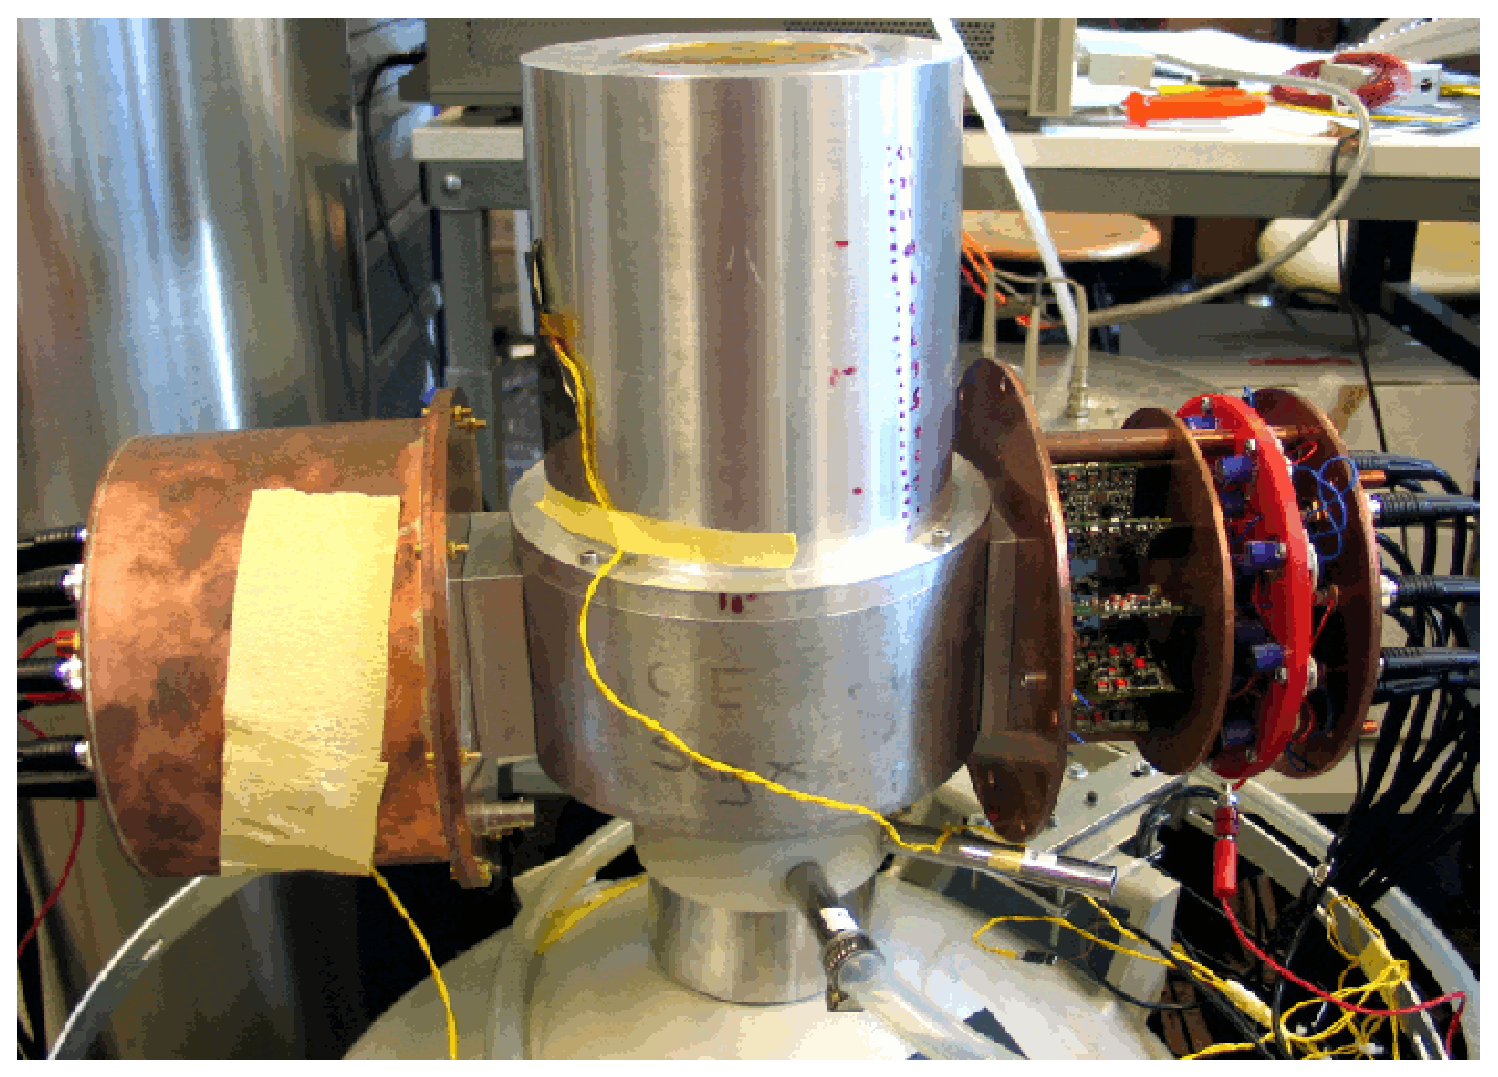
\includegraphics[height=0.25\textheight]{SIears}
  \caption{Left: commercial cryostat with \emph{Siegfried} I sitting     inside the top vacuum can. Right: a close-up to the vacuum can and     the copper ears housing pre-amplifier boards.}
  \label{fig:tt:comcryo}
\end{figure}

\subsection{Gerdalinchen II}
\label{sec:tt:gii}
Gerdalinchen II is a special cryostat manufactured in the technical division of Max-Planck-Institut f\"ur Physik for the test of operating several segmented germanium detectors directly in cryogenic liquid. As shown in the left drawing of Fig.~\ref{fig:tt:gii}, the main part of Gerdalinchen II is a two-walled cryogenic dewar sitting in a cylindrical aluminum tank with a hight of 960~mm and a diameter of 612~mm. The top flange can be lifted up vertically allowing mounting detectors to a vertical stainless steel bar under the flange and being lowered down into the dewar, as shown in the right picture of Fig.~\ref{fig:tt:gii}. The middle picture of Fig.~\ref{fig:tt:gii} shows the operation of a detector inside Gerdalinchen II with a neutron source placed aside. There are three high voltage feed-throughs and four signal connectors each with 18 channels on the top flange. This allows the operation of three 18-fold segmented detectors at the same time. The flange also contains tubes facilitating the re-filling of the dewar with cryogenic liquid, flashing with gaseous nitrogen and pumping without opening the system. The dewar is re-filled daily to prevent the cryogenic liquid level dropping down beneath the infrared shields (the thin copper tube and plate right above the detector as shown in Fig.~\ref{fig:tt:gii}). The liquid level is monitored by several thermal resistances (PT100) mounted in different places inside the dewar.

\begin{figure}[tbhp]
  \centering
  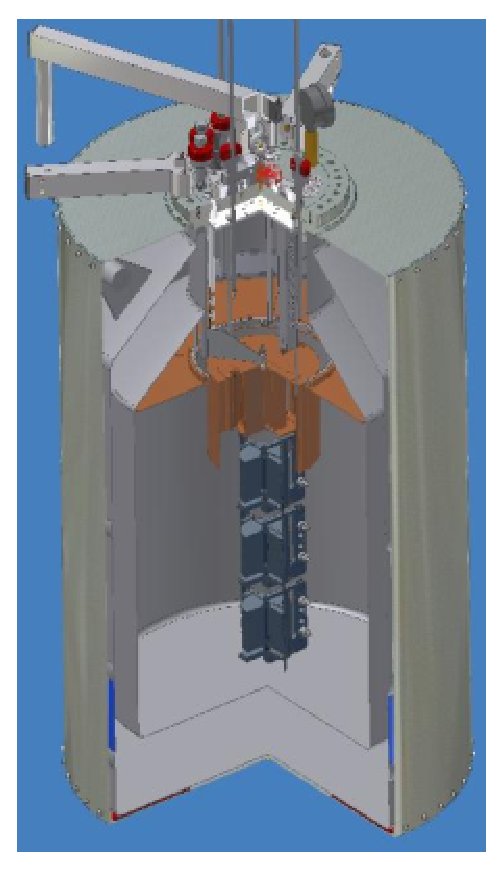
\includegraphics[height=0.25\textheight]{GIIdraw}\hfil
  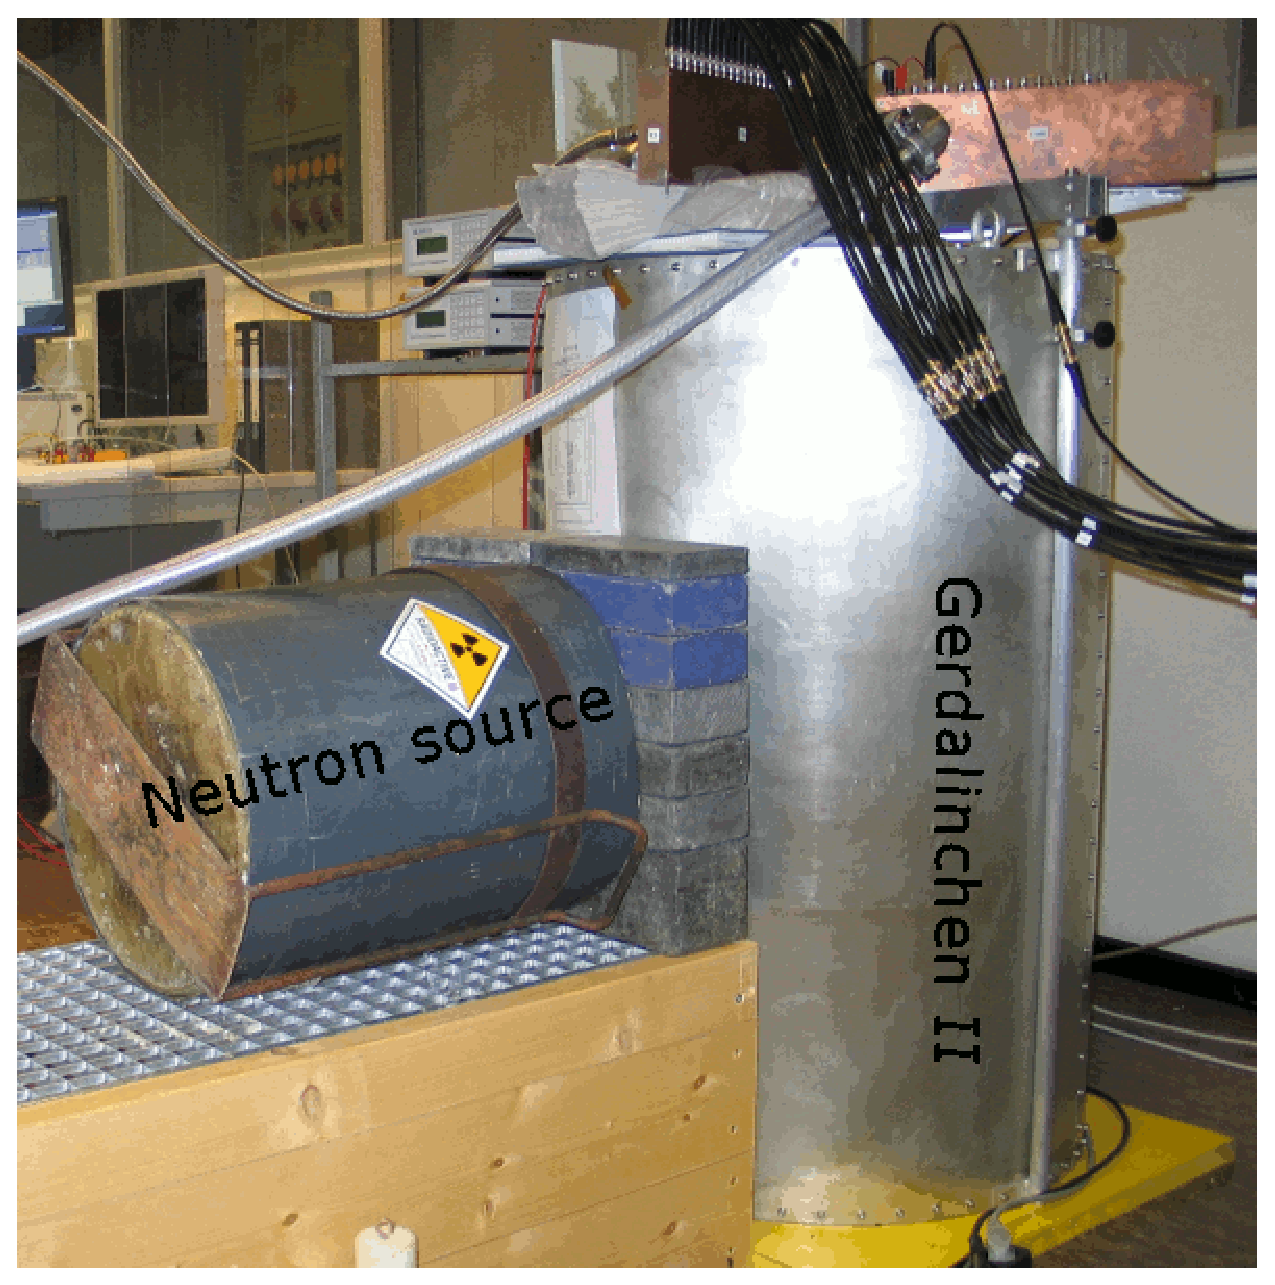
\includegraphics[height=0.25\textheight]{GIIneutron}\hfil
  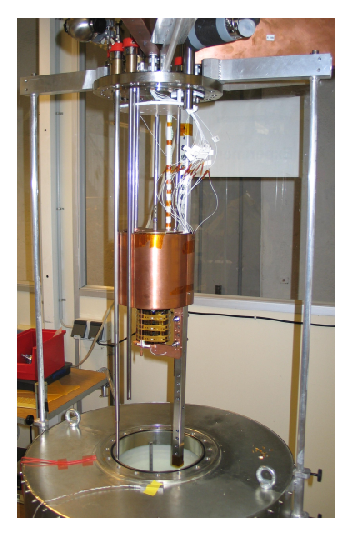
\includegraphics[height=0.25\textheight]{GIIdet}
  \caption{Left: technical drawing of Gerdalinchen II. Middle:     Gerdalinchen II in operation with a neutron source. Right:     Inserting a detector into Gerdalinchen II from the top.}
  \label{fig:tt:gii}
\end{figure}


\section{Electronics} 
\label{sec:tt:ele} 

\subsection{Front-end} 
\label{sec:tt:fend} 
A schematic diagram of \emph{Siegfried} I and its read out scheme are shown in the left plot of Fig.~\ref{fig:tt:sif}. The signals were read out using charge sensitive PSC-823C pre-amplifiers with a decay time of 50~$\mu$s. The FET for the core electrode was mounted inside the cryostat close to the detector, the FETs for the segment electrodes were incorporated into the pre-amplifier boards which were housed in the copper ears on both sides of the detector as shown in the right picture of Fig.~\ref{fig:tt:comcryo}. The right plot of Fig.~\ref{fig:tt:sif} shows the layout of the feed-throughs to \emph{Siegfried} I. They are placed on the end caps of the copper ears.

\begin{figure}[tbhp]
  \centering
  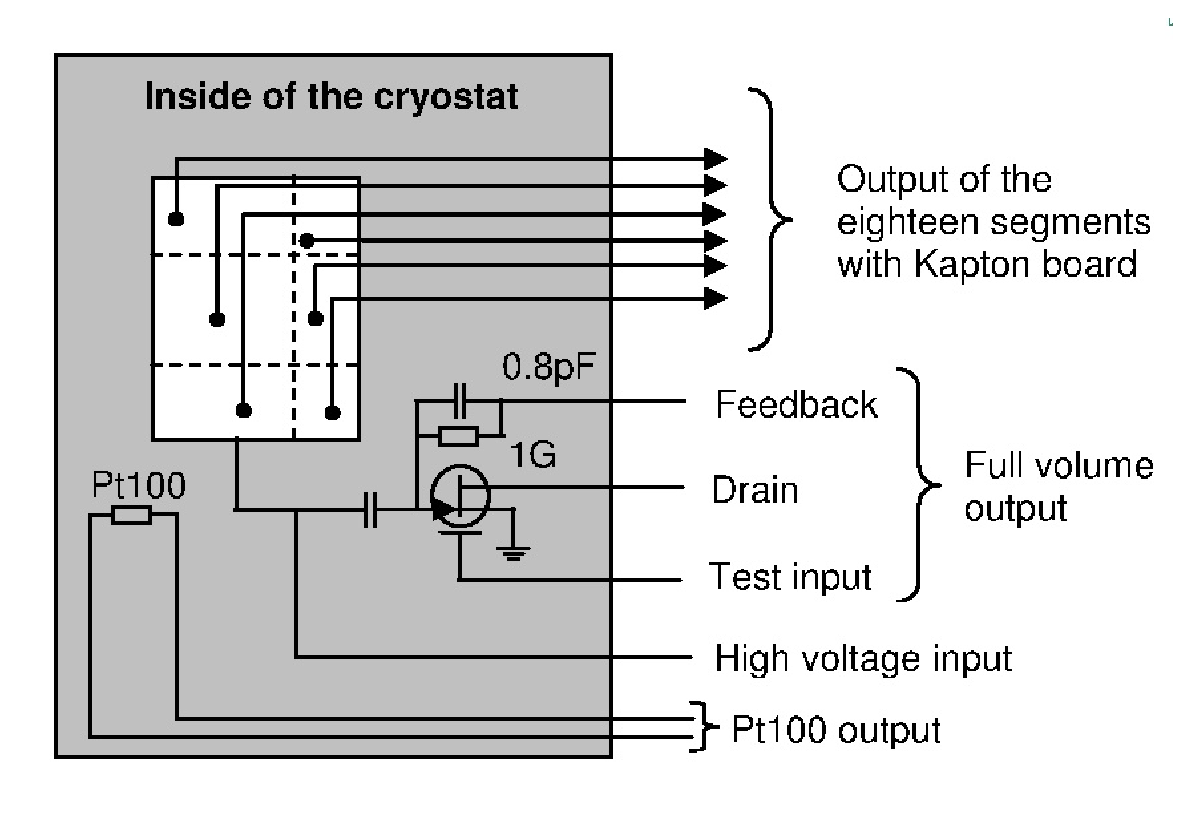
\includegraphics[height=0.25\textheight]{block1}\hfil
  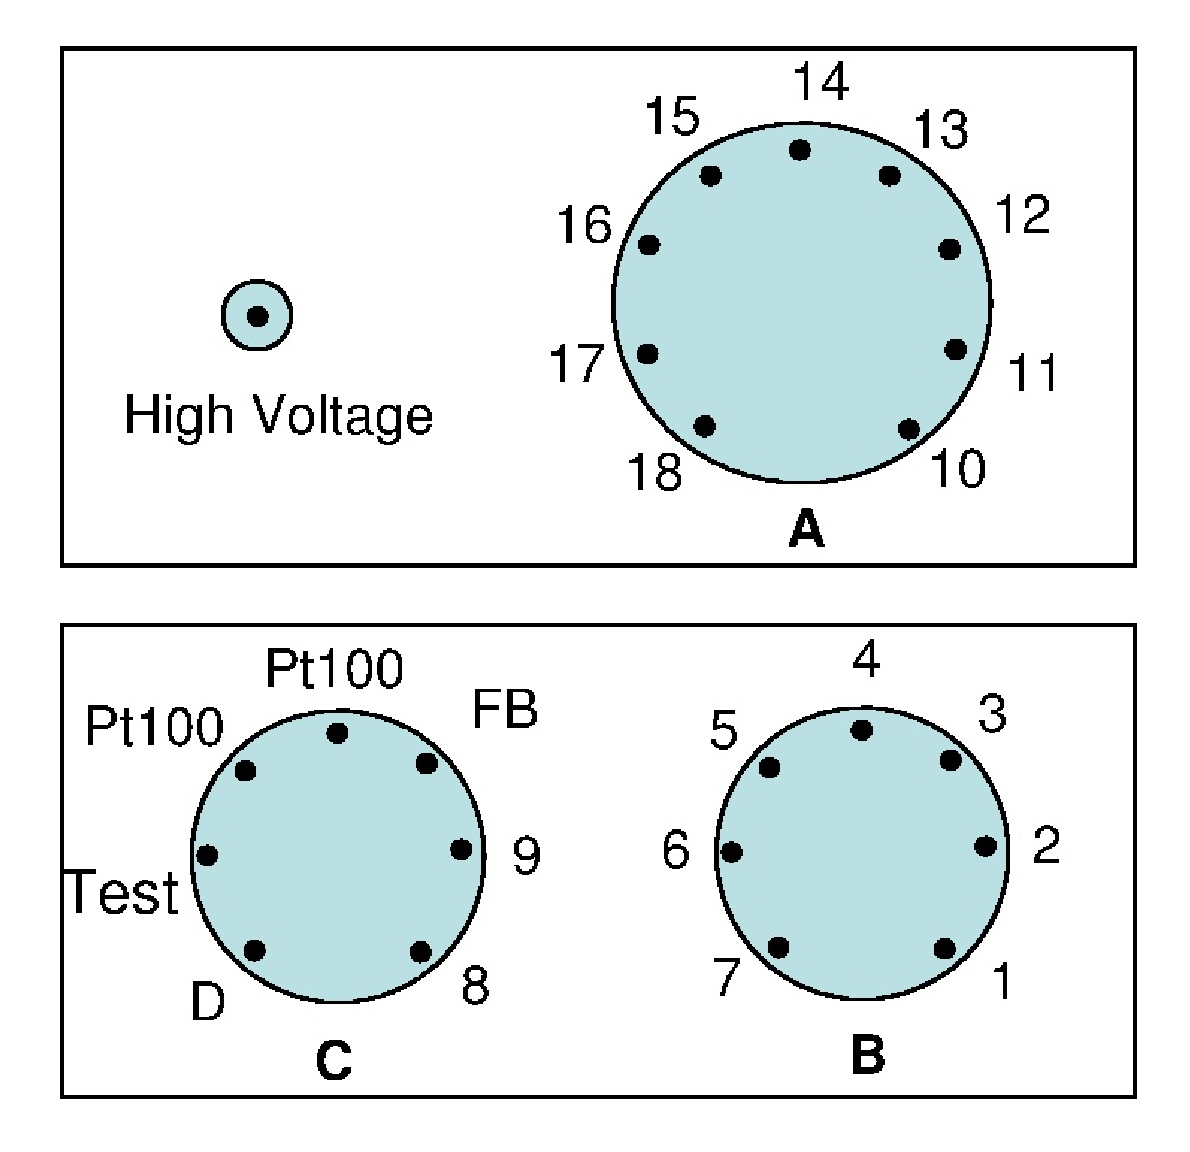
\includegraphics[height=0.25\textheight]{block2}
  \caption{Schematic diagram of \emph{Siegfried} I and its read out     scheme (left) and the layout of the feed-throughs to the     commercial cryostat (right).}
  \label{fig:tt:sif}
\end{figure}

For the operation of detectors in Gerdalinchen II a different setup was used. The FET for the core electrode was incorporated into the pre-amplifier boards like the segment electrodes. The core signal was not amplified before the pre-amplifier board, the cross talks to the segment signals from the core signal was minimized. All the pre-amplifier boards were mounted in a copper box and shared a common ground as shown in the right picture of Fig.~\ref{fig:tt:gef}. The noise filter for the high voltage lines and the coupling capacitors for the core signal cables were placed under the top flange as shown in the left picture of Fig.~\ref{fig:tt:gef}. They were operated above the cryogenic liquid level and moved later below the level for better temperature stability.
\begin{figure}[tbhp]
  \centering
  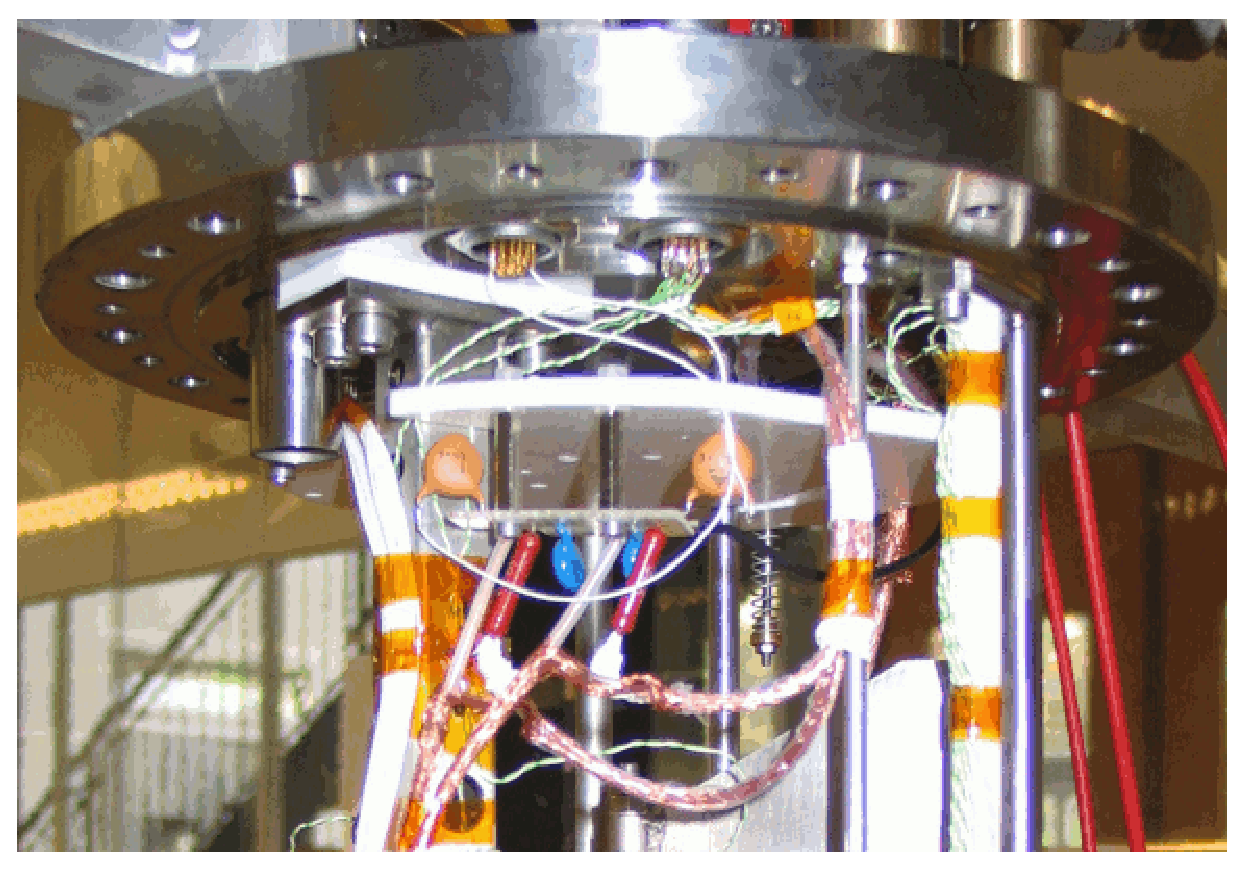
\includegraphics[height=0.2\textheight]{GIIHV}\hfil
  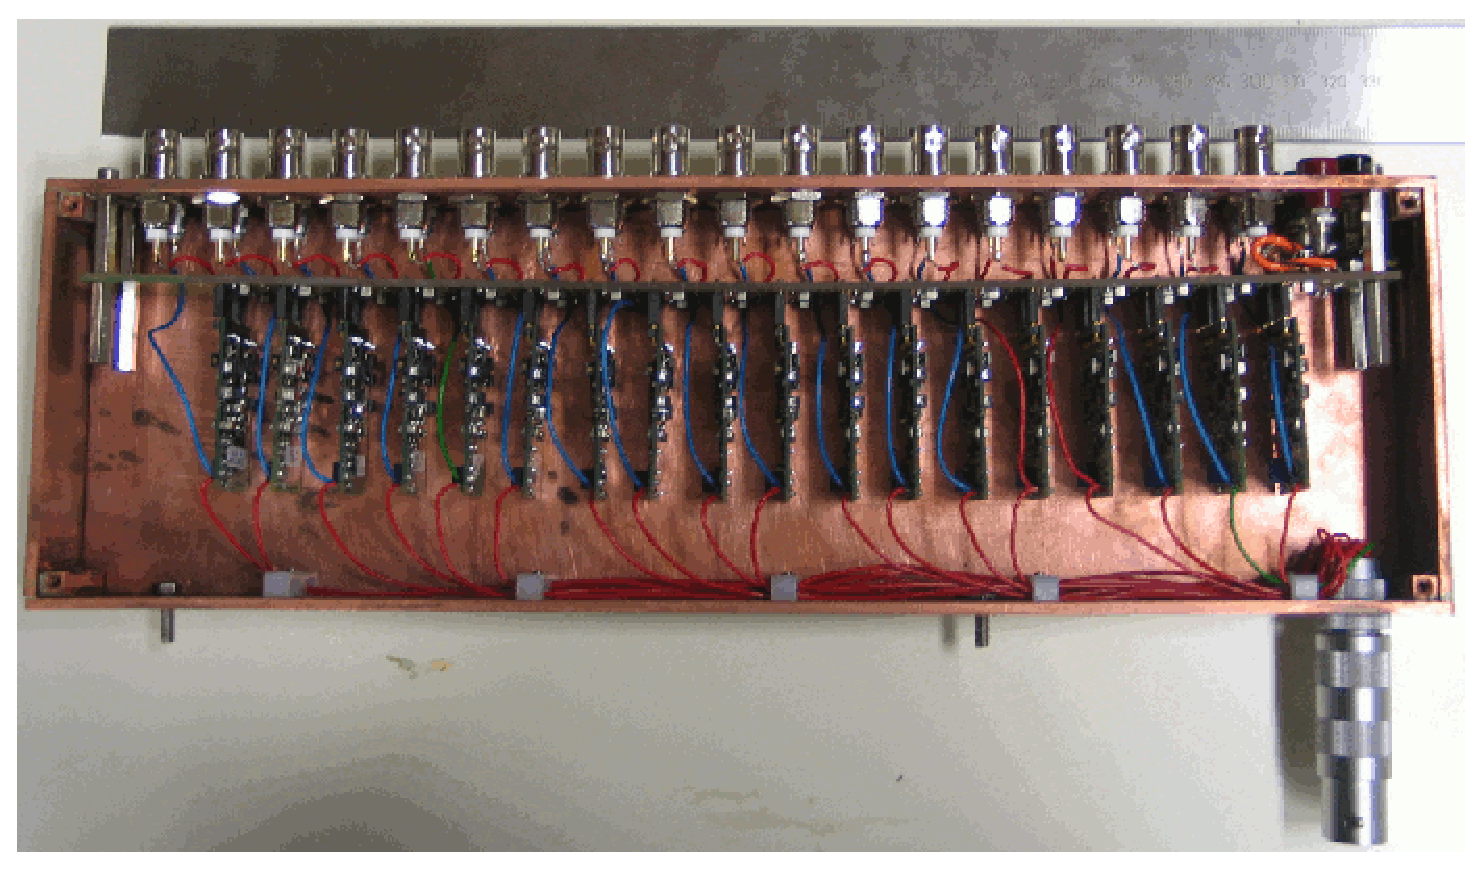
\includegraphics[height=0.2\textheight]{GIIpreamp}
  \caption{Left: high voltage filter and coupling capacitor in     Gerdalinchen II. Right: pre-amplifier box for one segmented     detector in Gerdalinchen II.}
  \label{fig:tt:gef}
\end{figure}

\subsection{DAQ} 
\label{sec:tt:daq}
The pre-amplified signals are digitized using a data acquisition system based on 5 14-bit ADC PIXIE-4 modules at a sampling rate of 75~MHz. The bandwidth of analog signals is limited by a Nyquist filter to half the sampling rate, \textit{i.e.} 37.5~MHz. This avoids aliasing in the noise from higher frequencies. It is implemented in the analog section of the PIXIE-4 module, with a low-pass Sallen-Key filter that makes a sharp (but finite) cut-off at this frequency. Energy is calculated using software filters~\cite{Pixie4}. Recorded pulse shape data consist of 300 samples of the integrated charge amplitude. The onset of the signal can be set by hand and was set to 1~$\mu$s for most of the measurements. The trigger and energy thresholds of the core and segment electrodes can be set to different values. The pile-up pulses can be rejected or recorded with a rough estimation of the energy.

\section{Accessories} 
\label{sec:tt:lamo}
The accessory equipments relevant to the operation of test facilities include high voltage supplies, temperature monitors, vacuum gauges, oxygen sensors, etc. Variables given by these equipments need to be monitored, recorded and analyzed in order to ensure a successful measurement. For overnight or long term measurements these monitoring processes need to be automated. A generalized Laboratory Monitor system, LaMo, has been developed to monitor and control most of the hardware in the laboratories using the graphic programming language, LabVIEW. The aim of the project is to create a slow control framework with a set of user friendly interfaces for most of the common lab tasks and to speed up the implementation of new pieces of hardware.

Fig.~\ref{fig:tt:lamo} shows the main panels of LaMo. The first panel one can see when opening LaMo is called ``laboratory'' as shown in the left screen shot of Fig.~\ref{fig:tt:lamo}. It shows a list of experiments going on in the laboratory and their status. An experiment can be created, edited, started, stopped using the bottoms aside the experiment list. The ``laboratory'' panel also provides functions common for all experiments, such as email alerts, power supply, oxygen sensors, etc. Different pieces of hardware relevant to an experiment can be chosen from a list of available hardware. This is done in the ``edit'' panel of LaMo as shown in the middle screen shot of Fig.~\ref{fig:tt:lamo}, where different hardware can be added, deleted from the equipment list for monitoring. Once an experiment is created and configured, it can be run by click the start bottom in ``laboratory'' panel. An ``experiment'' panel, as shown in the right screen shot of Fig.~\ref{fig:tt:lamo}, will be brought up, where monitored variables are shown in different ways. The functions specified for a particular experiment can be accessed from here.

\begin{figure}[tbhp]
  \centering
  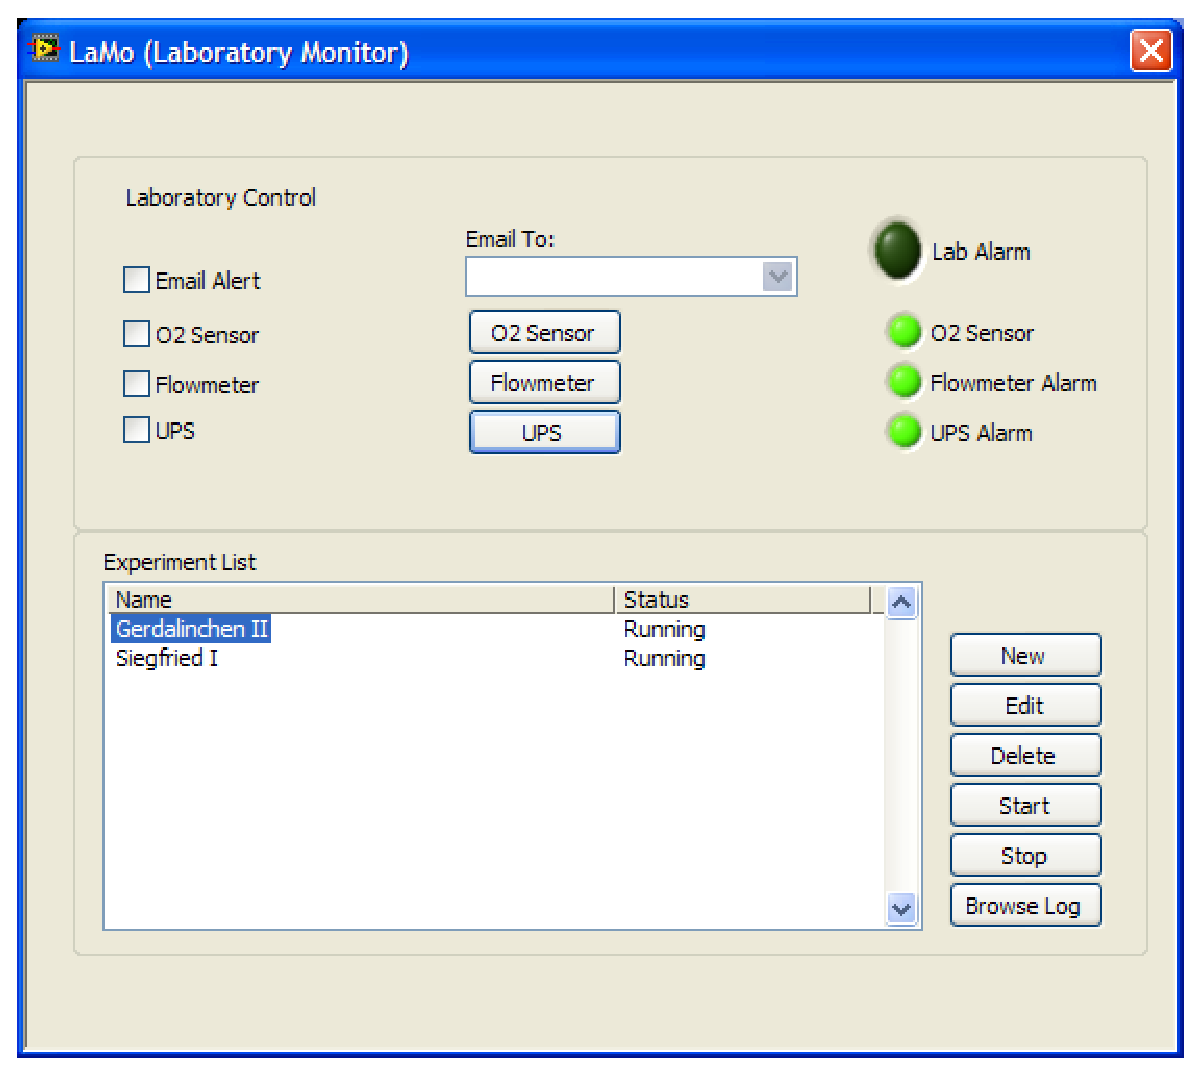
\includegraphics[height=0.23\textheight]{LaMoLab}\hfil
  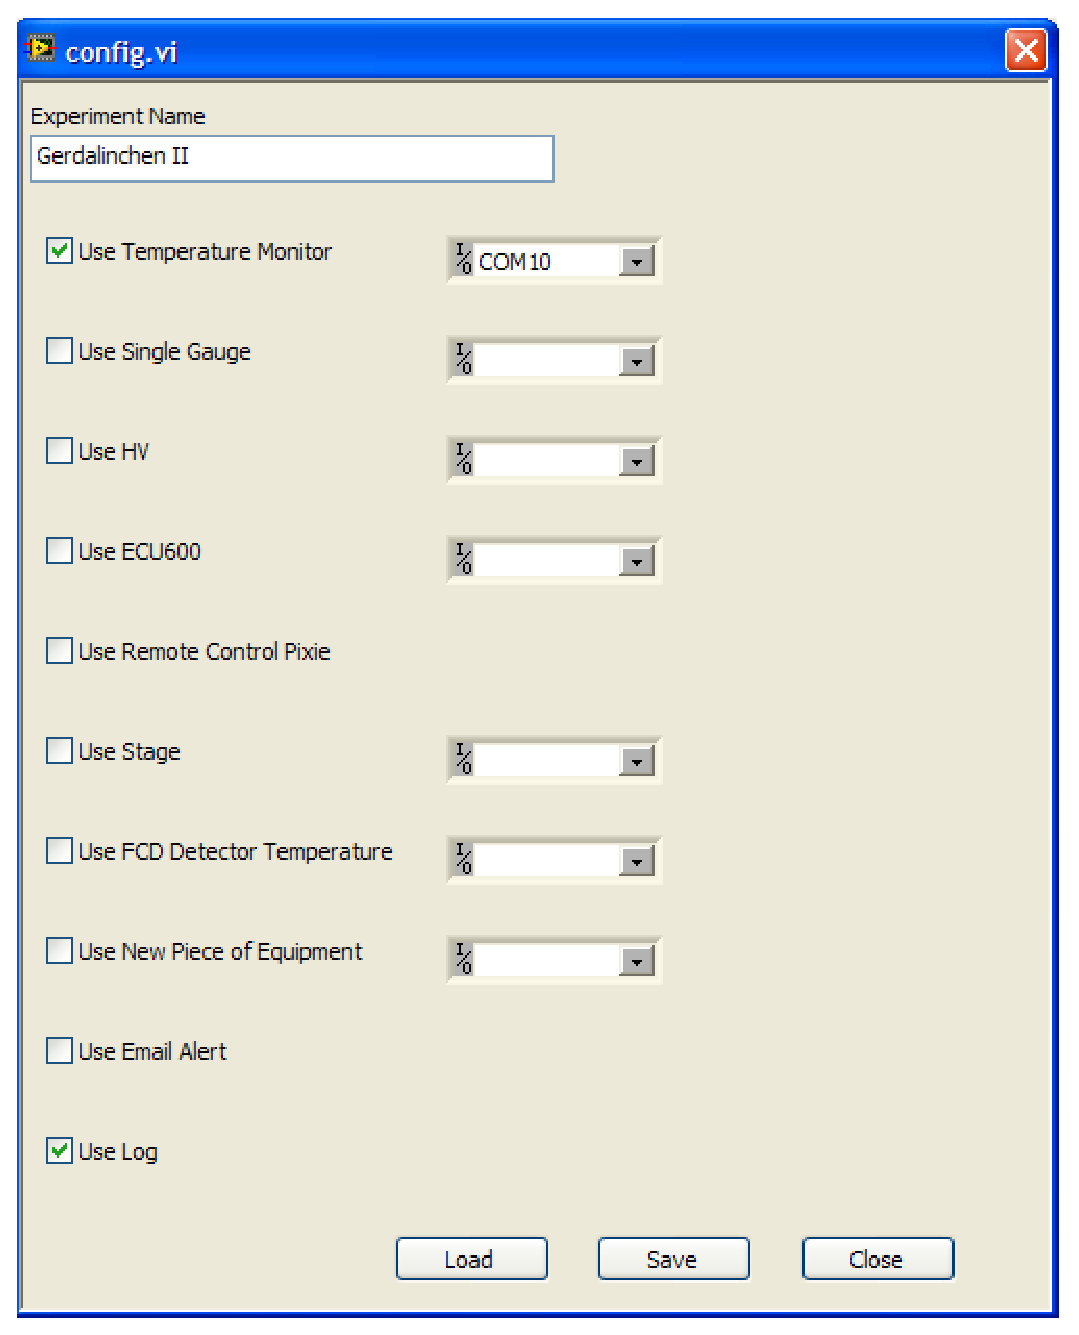
\includegraphics[height=0.23\textheight]{LaMoEdit}\hfil
  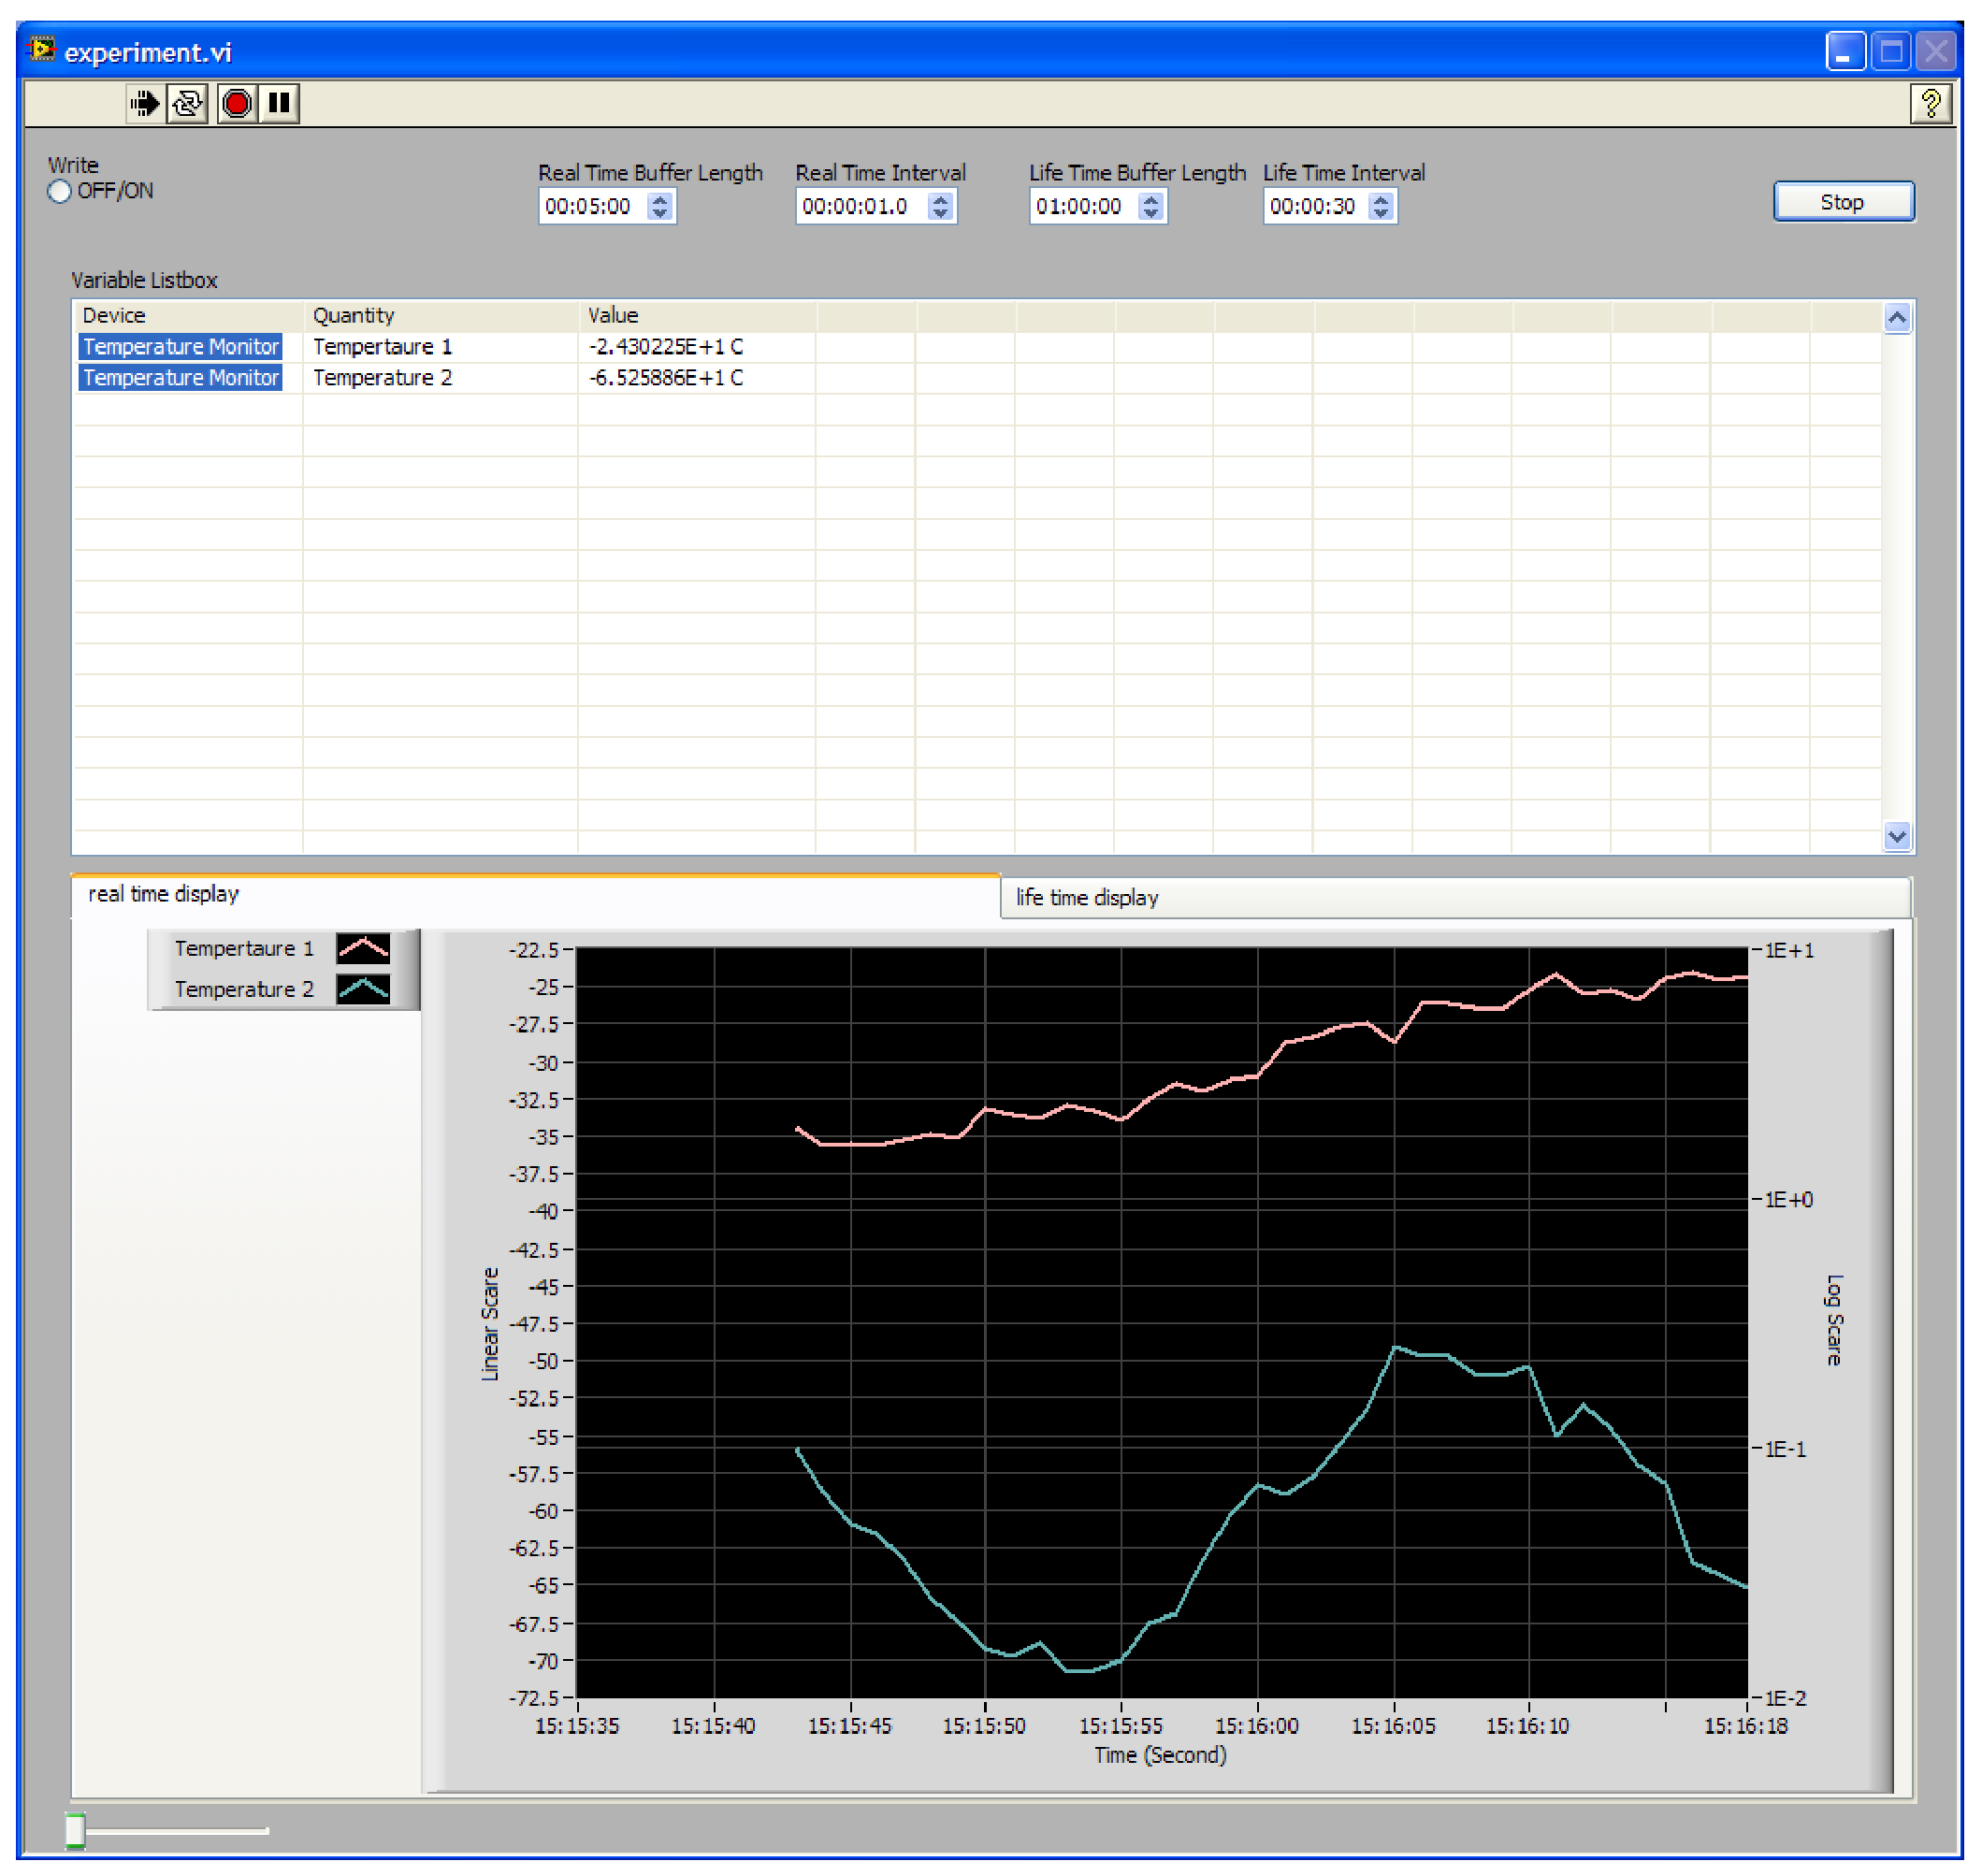
\includegraphics[height=0.23\textheight]{LaMoExp}
  \caption{Left: laboratory panel of LaMo, showing list of experiments     and their status, and giving access to functions common for all     experiments. Middle: edit panel of LaMo, where pieces of hardware     relevant to an experiment can be added/deleted from the equipment     list for monitoring. Right: experiment panel of LaMo, where     monitored variables can be shown in different ways. The functions     specified for a particular experiment can be accessed here.}
  \label{fig:tt:lamo}
\end{figure}

The common user interface enforces common I/Os for different pieces of hardware. The functionality of LaMo is modularized so that the effort to implement a new piece of hardware is minimized. To add a new equipment the developer only needs to define its I/O interface to LaMo. The other efforts, such as programming the user interface, etc., need not to be repeated every time.

\section{Monte Carlo simulation} 
\label{sec:tt:sim}
Monte Carlo simulations of prototype detectors and their cryostats was performed using MaGe~\cite{Mag08}, a C++ package co-developed by the Majorana and GERDA collaborations using Geant4 toolkits~\cite{Gea03,Gea06}. Figure~\ref{fig:tt:sim} shows the geometry models of the detectors and cryostats implemented in Geant4. The right plot of Fig~\ref{fig:tt:sim} shows a close-up of the \emph{Siegfried} II geometry. It was modeled in such a way that the details were implemented as close as possible to reality while the simulation efficiency did not decrease too much.

The energy depositions of hits in each segment were recorded and the core energy was calculated by adding all segment energies. The segment and core energies were individually smeared according to the energy resolutions of the detectors measured in the individual channels.

The spacial and time information of hits were also recorded, which served as parts of the input for the pulse shape simulation package. The geometry of detectors and the voltage bias applied were other input information for the pulse shape simulation. The detail of the pulse shape simulation is described in Chapter~\ref{cha:pss}.
 
\begin{figure}[tbhp]
  \centering
  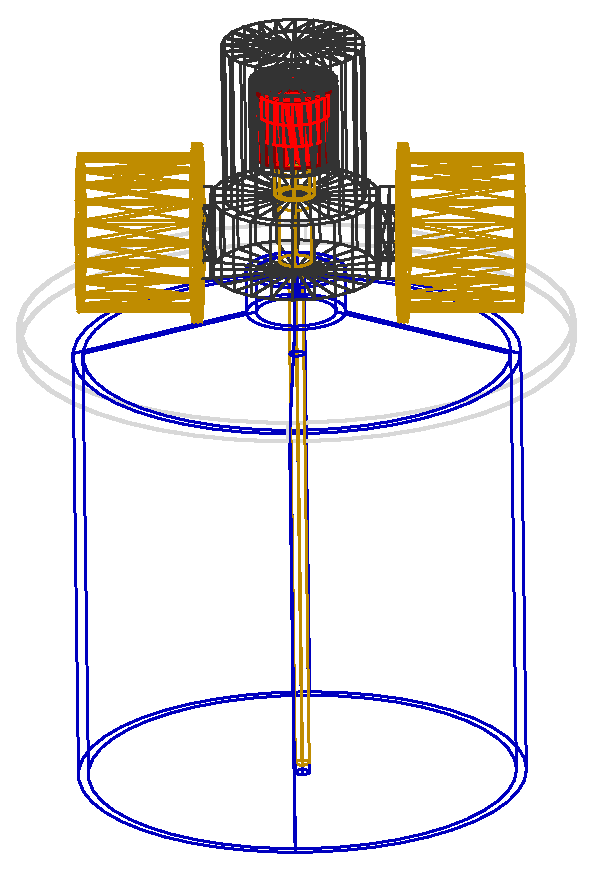
\includegraphics[height=0.3\textheight,clip]{SIwired}\hfil
  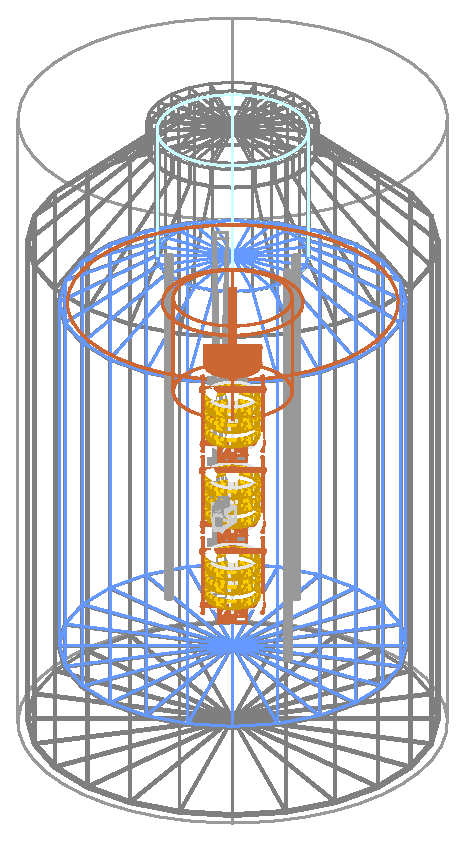
\includegraphics[height=0.3\textheight,clip]{GIIwired}\hfil
  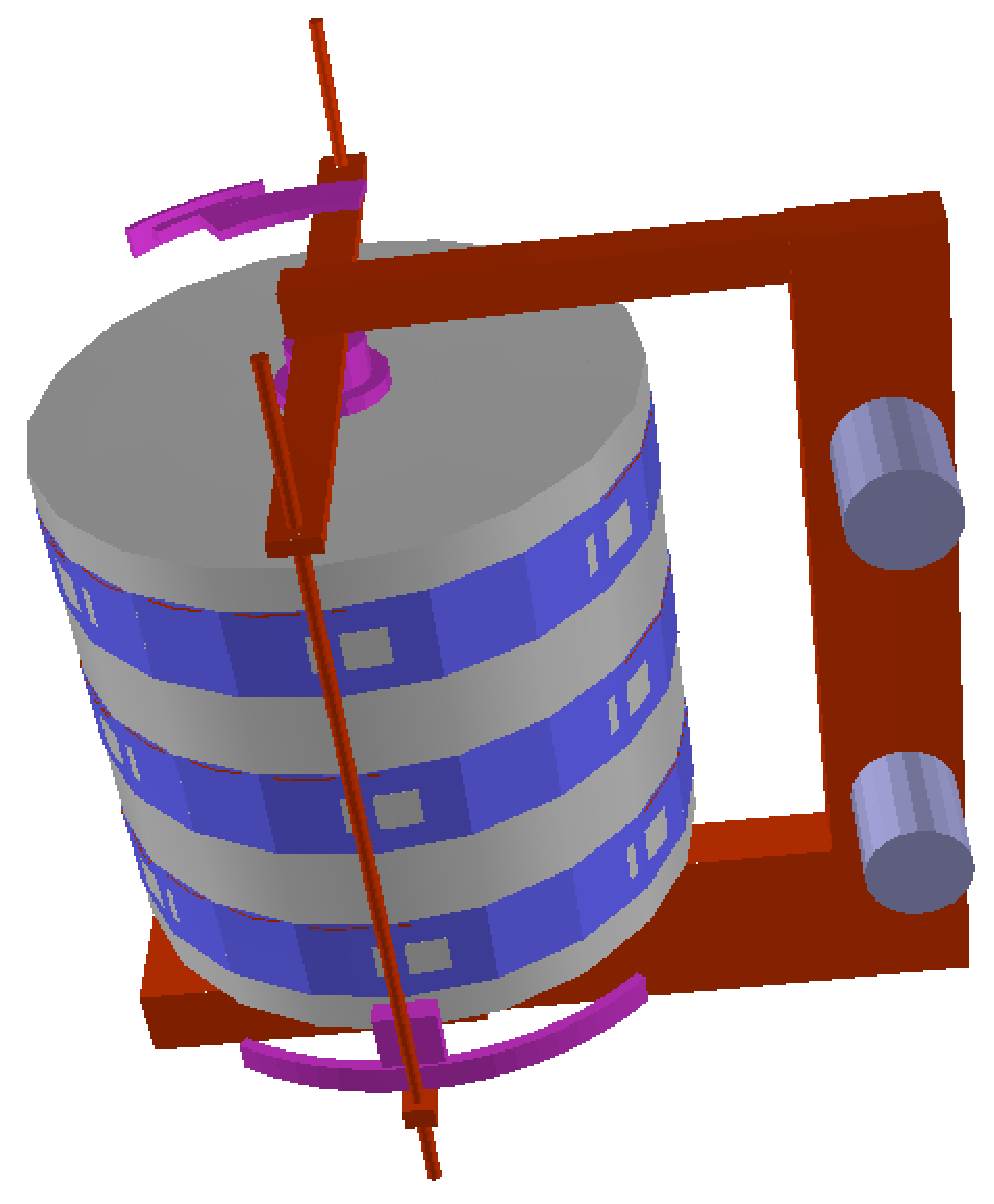
\includegraphics[height=0.3\textheight,clip]{SIIsolid}
  \caption{Left: wired drawing of the commercial cryostat geometry.     Middle: wired drawing of Gerdalinchen II geometry. Right: a     close-up of \emph{Siegfried} II geometry with copper supporting     frame as used in Gerdalinchen II.}
  \label{fig:tt:sim}
\end{figure}


%%% Local Variables:
%%% mode:latex
%%% TeX-master: "thesis"
%%% End:
